\chapter[L'application]{Présentation de l'application}

Dans ce chapitre on présente l'application Crazy wolf. 
Au traver d'images commentées nous allons décrire plusieurs scénarios
d'utilisation.
\section{Scénario I}
\subsection*{Authentification \& écran d'accueil}
Ici la serveuse Kim, qui n'a pas de privilèges, c'est-à-dire qu'elle n'est 
ni manager ni administratice, se connecte et accède au premier écran possible.
Puis elle, click sur "Mes services".

\begin{figure}[!h]
    \centering
    \begin{subfigure}{.3\textwidth}
        \centering
        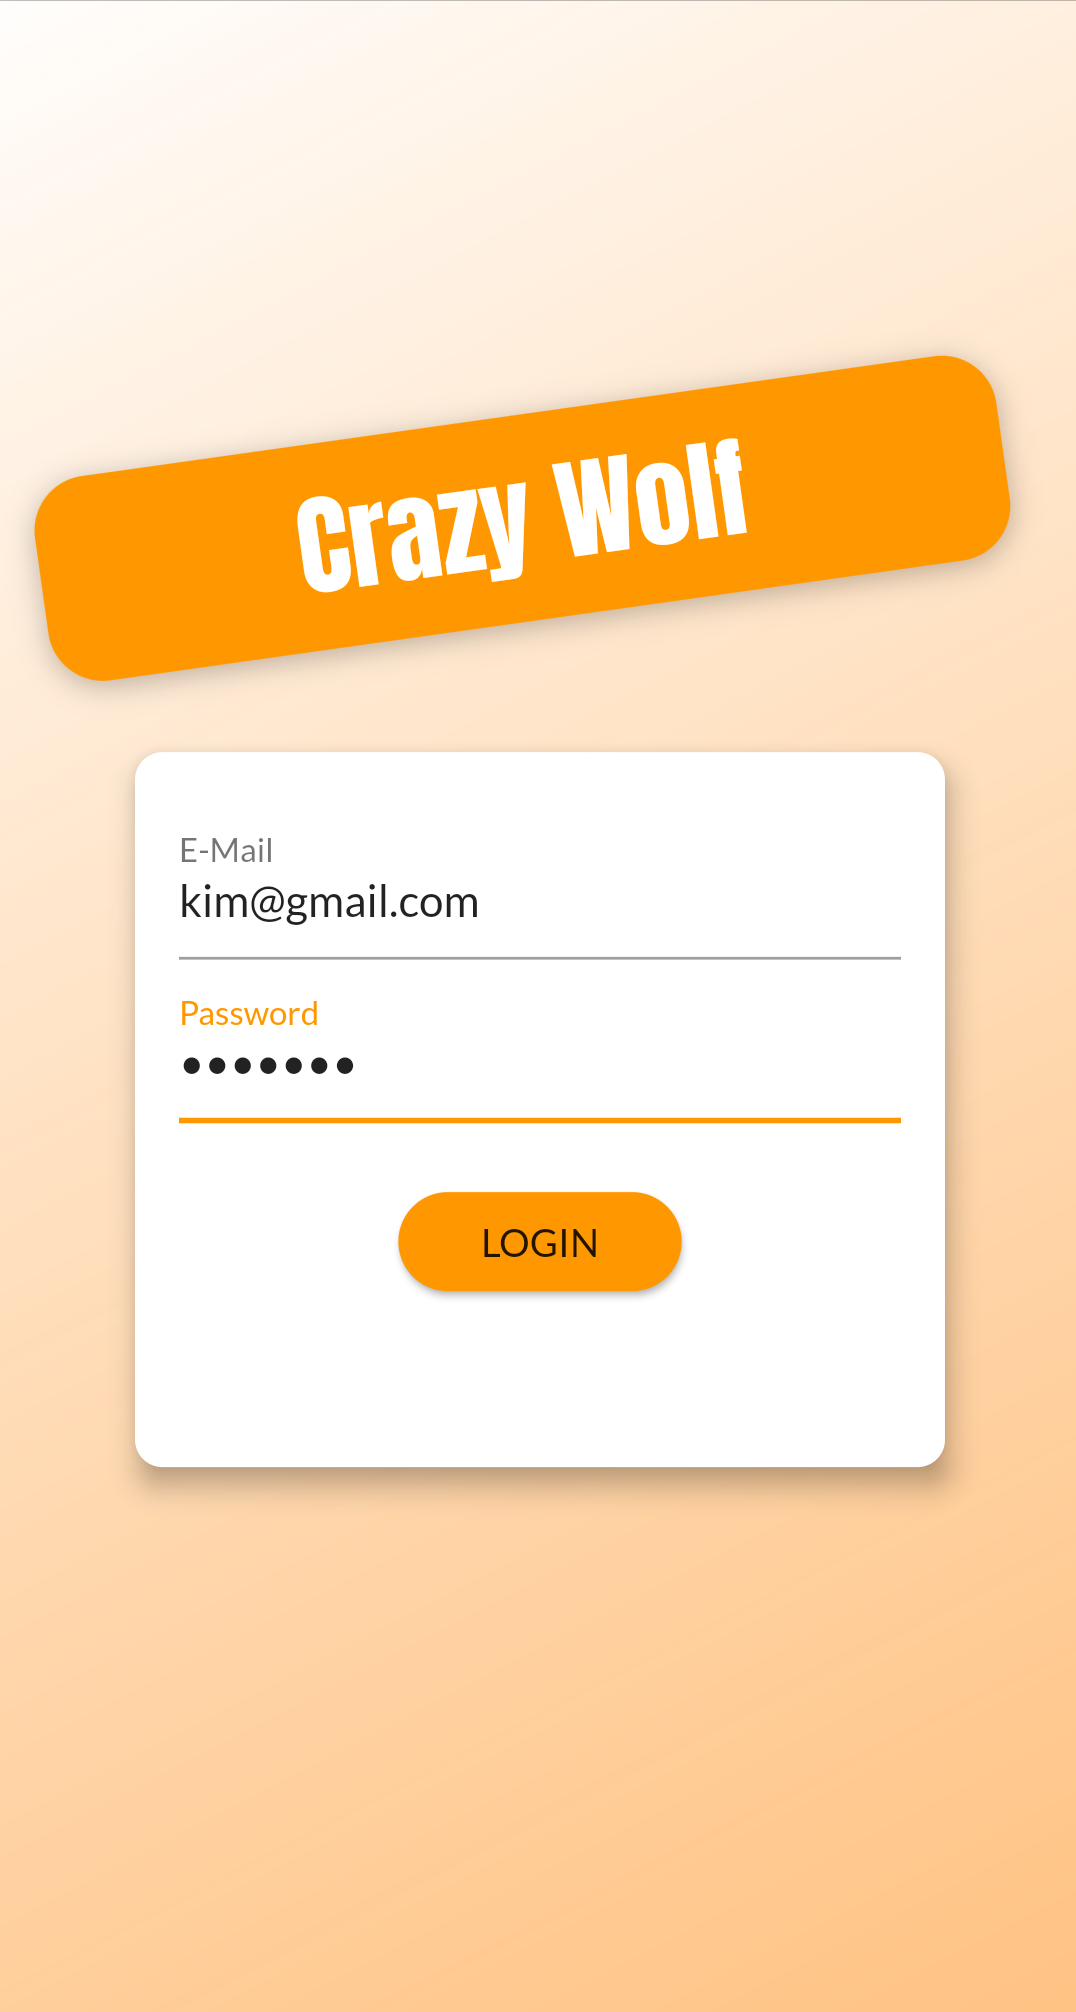
\includegraphics[width=0.9\linewidth]{screenshots/scenario_01/login.png}
        \caption{login}
        \label{fig:login}
    \end{subfigure}
    \begin{subfigure}{.3\textwidth}
        \centering
        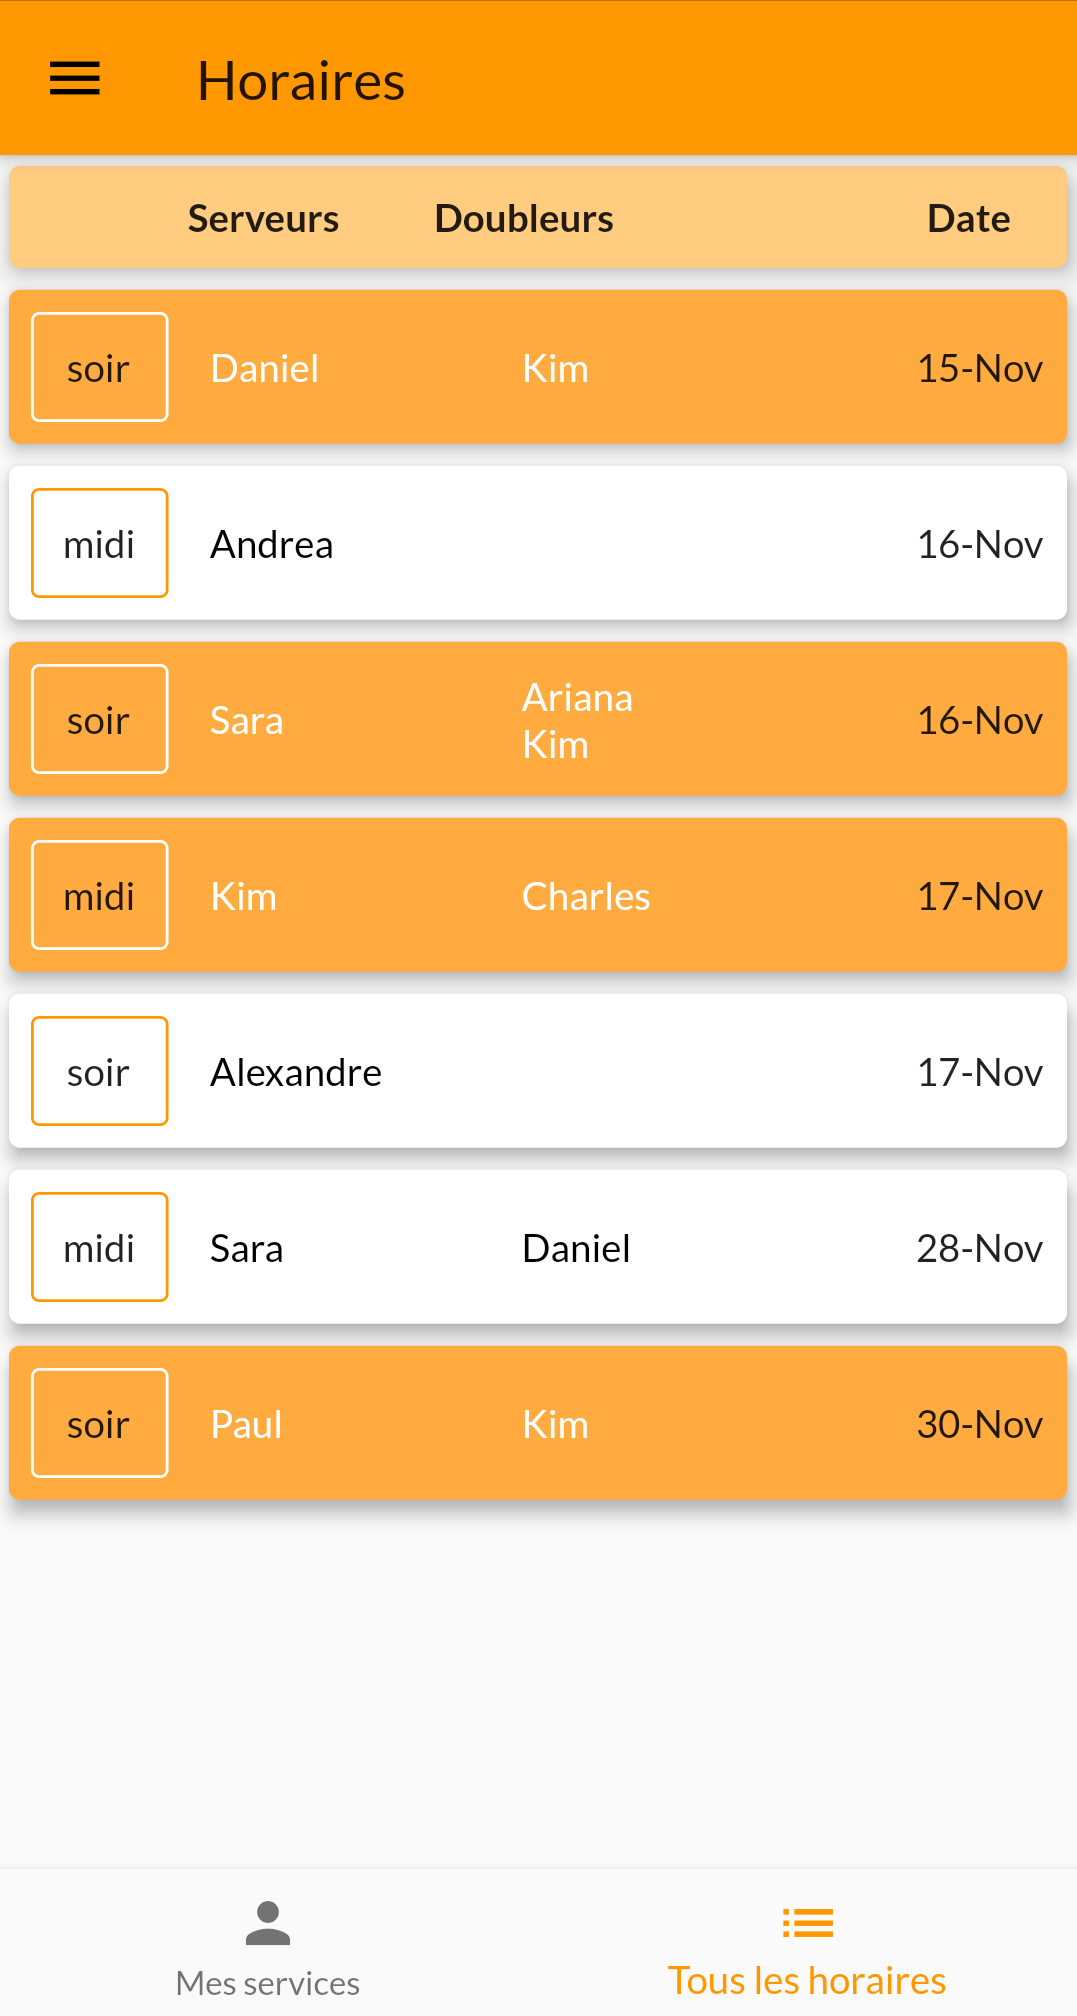
\includegraphics[width=0.9\linewidth]{screenshots/scenario_01/horaires.png}
        \caption{horaires}
        \label{fig:horaires}
    \end{subfigure}
    \begin{subfigure}{.3\textwidth}
        \centering
        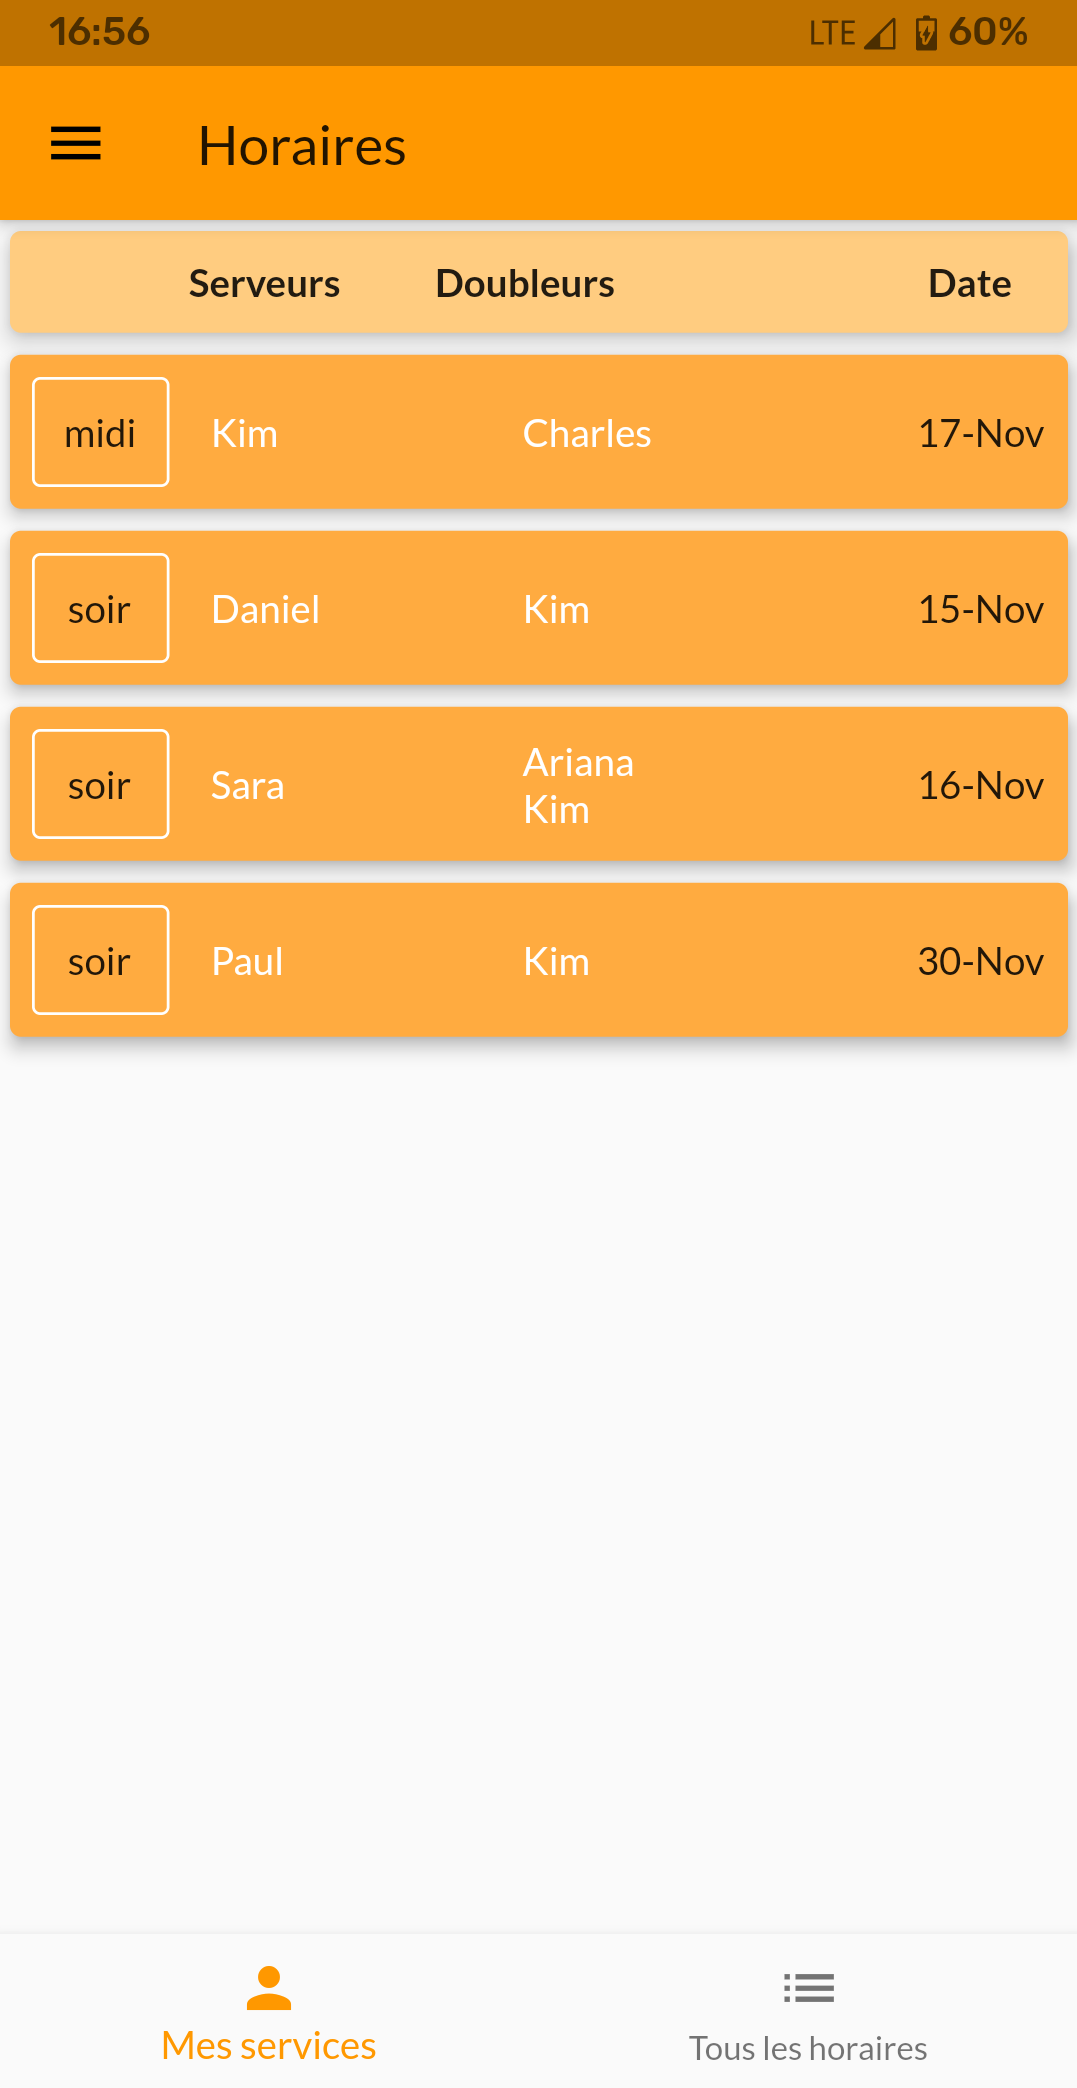
\includegraphics[width=0.9\linewidth]{screenshots/scenario_01/mesHoraires.png}
        \caption{mes horaires}
        \label{fig:mesHoraires}
    \end{subfigure}
    \caption{scénario I}
    \label{fig:scen01}
\end{figure}

L'utilisateur doit dans un premier temps se connecter à l'aide d'identifiants déjà existant dans l'écran \ref{fig:login}. Une fois l'addresse mail et le mot de passe saisis, 
l'écran \ref{fig:horaires} s'affiche. 

On y voit l'ensemble des horaires de travail. Il sont identifié par un type: midi ou soir, par un ou plusieurs 
serveurs, par un ou plusieurs doubleurs et par une date. Les services sont affichés par dates.
Les jours précédents au moment de la connection ne 
sont pas affichés. Les horaires correspondant à la personne authentifié sont de couleurs orange.

On peut également naviguer à l'aide du menu inférieur à "mes services" où seuls les horaires du serveur authentifié sont affichés. Comme on le voit 
dans \ref{fig:mesHoraires}

\section{Scénario II}
    \subsection*{Mise en bourse d'un service}
    Supposons que la serveus Kim authentifiée ne puisse pas travailler le 17 novembre.
    Praesent in sapien. Lorem ipsum dolor sit amet, consectetuer 
adipiscing elit. Duis fringilla tristique neque. Sed interdum 
libero ut metus. Pellentesque placerat. Nam rutrum augue a leo. 
Morbi sed elit sit amet ante lobortis sollicitudin.
\section{Scénario III}
Praesent in sapien. Lorem ipsum dolor sit amet, consectetuer 
adipiscing elit. Duis fringilla tristique neque. Sed interdum 
libero ut metus. Pellentesque placerat. Nam rutrum augue a leo. 
Morbi sed elit sit amet ante lobortis sollicitudin.

Praesent in sapien. Lorem ipsum dolor sit amet, consectetuer 
adipiscing elit. Duis fringilla tristique neque. Sed interdum 
libero ut metus. Pellentesque placerat. Nam rutrum augue a leo. 
Morbi sed elit sit amet ante lobortis sollicitudin.

Praesent in sapien. Lorem ipsum dolor sit amet, consectetuer 
adipiscing elit. Duis fringilla tristique neque. Sed interdum 
libero ut metus. Pellentesque placerat. Nam rutrum augue a leo. 
Morbi sed elit sit amet ante lobortis sollicitudin.
\section{Scénario IV}
Praesent in sapien. Lorem ipsum dolor sit amet, consectetuer 
adipiscing elit. Duis fringilla tristique neque. Sed interdum 
libero ut metus. Pellentesque placerat. Nam rutrum augue a leo. 
Morbi sed elit sit amet ante lobortis sollicitudin.

Praesent in sapien. Lorem ipsum dolor sit amet, consectetuer 
adipiscing elit. Duis fringilla tristique neque. Sed interdum 
libero ut metus. Pellentesque placerat. Nam rutrum augue a leo. 
Morbi sed elit sit amet ante lobortis sollicitudin.
Praesent in sapien. Lorem ipsum dolor sit amet, consectetuer 
adipiscing elit. Duis fringilla tristique neque. Sed interdum 
libero ut metus. Pellentesque placerat. Nam rutrum augue a leo. 
Morbi sed elit sit amet ante lobortis sollicitudin.


Praesent in sapien. Lorem ipsum dolor sit amet, consectetuer 
adipiscing elit. Duis fringilla tristique neque. Sed interdum 
libero ut metus. Pellentesque placerat. Nam rutrum augue a leo. 
Morbi sed elit sit amet ante lobortis sollicitudin.

